\documentclass[a4paper, 11pt]{article}

\usepackage[utf8]{inputenc}
\usepackage[IL2]{fontenc}
\usepackage[slovak]{babel}
\usepackage[unicode]{hyperref}
\usepackage{graphics}
\usepackage{graphicx}
\usepackage{pdflscape}
\usepackage{ragged2e}
\usepackage[dvipsnames]{xcolor}
\usepackage[left = 2cm, top = 3cm, total={17cm, 24cm}]{geometry}
\usepackage{listings}

\begin{document}

\begin{titlepage}
    \begin{center}
        \includegraphics{fit.pdf}
        
        \vspace{\stretch{0.382}}
        \Huge{Klasifikátor hodnotenia kvality obrazu sietnice} \\
        \LARGE{Dokumentácia k projektu BIO}
        \vspace{\stretch{0.618}}
    \end{center}
        {\Large \today \hfill Bc. Tomáš Ondrušek(xondru18)} \\
    
    \begin{FlushRight}
        \Large Bc. Peter Ďurica(xduric05)
    \end{FlushRight}
\end{titlepage}

\tableofcontents
\pagebreak

\section{Úvod}
Táto práca sa zaoberá automatickým hodnotením kvality snímkov sietnice využitím neurónových sietí. Sietnica \cite{OCY_veducko} je tenká, polopriehľadná, viacvrstvová časť neurálneho tkaniva. Pokrýva dve tretiny vnútra každého oka. Má za úlohu konvertovať elektromagnetický signál z vonku do neurónového signálu, ktorý následne odovzdá optickému nervu.

Kvôli architektúre sietnice \cite{RetImag} je možné v jej snímkach zachytiť choroby oka alebo aj choroby mozgu a cirkulácie krvy. Vďaka analýze snímkov je možné tieto choroby správne identifikovať a nariadiť účinnú liečbu pre pacienta.

Zlá kvalita sietnicových obrázkov \cite{OCY_veducko} môže zvýšiť pravdepodobnosť zlej diagnózy alebo sponzorovania choroby. Takisto môže spôsobiť predĺženie stráveného času pri analýze snímkov. Napríklad rozmazané obrázky môžu zakryť poškodené cievy v sietnici a tým pádom sa môže daná sietnica výskumníkom javiť ako zdravá. Automatická kontrola a identifikácia kvality snímkov môže proces analýzy spresniť a urýchliť. Výsledkom bude väčšia bezpečnosť pacientov a zvýšený komfort zdravotníkov.



\section{Hodnotenie kvality obrazu sietnice}
Sietnicu je možné odfotiť pomocou fundus fotoaparátu. Následné fotografie sa vedia analyzovať a podľa tej analýzy vyhodnotiť zdravie sietnice na obrázku. Táto kapitola sa zaoberá štruktúrou sietnice a hodnotením kvality fotografie.
\subsection{Fotografia sietnice}
Na obrázku \ref{fig:retina_struct} je zobrazená fotografia sietnice oka. Na snímke je vidno \cite{OCY_veducko} stromovú štruktúru centrálnej sietnicovej tepny (angl. Central Retinal Artery) a centrálnej sietnicovej žily (angl. Central Retinal Vein). Spolu tvoria štruktúru krvných ciev na sietnici.

Ďalšie anatomické štruktúry \cite{OCY_veducko}, ako žltá škvrna (angl. Macula), fovea, optický disk (angl. Optic Disk) a optický pohár (angl. Optic Cup) by mali byť rovnako jasne identifikovateľné na dobre zosnímanom obrázku sietnice.

\medskip\noindent Pozorovaním týchto oblastí sietnice je možné spozorovať niektoré choroby \cite{RetImag} napríklad:
\begin{itemize}
    \item \textbf{Diabetická retinopatia} - Zmeny na cievach sietnice,
    \item \textbf{Makulárna degenerácia} - Zmeny v oblasti žltej škvrny,
    \item \textbf{Glaukóm} - Zmeny v optickom nerve alebo v cievach.
\end{itemize}

\begin{figure*}[b!]
    \centering
    \includegraphics[width=0.3285\linewidth]{images/retina_struct.png}
    \caption{Fotografia štruktúr sietnice oka \cite{OCY_veducko}}
    \label{fig:retina_struct}
\end{figure*}
\subsection{Kategórie kvality snímkov}

\begin{figure*}[t!]
    \centering
    \includegraphics[width=0.7\linewidth]{images/quality_levels.png}
    \caption{Rozdelenie fotografií sietnice oka podľa kvality \cite{OCY_cinan}}
    \label{fig:quality levels}
\end{figure*}

Kvalita fotiek sietnice \cite{OCY_cinan} sa delí do troch kategórií:

\begin{itemize}
    \item \textbf{Good} - Ideálna výsledná kvalita fotografie,
    \item \textbf{Usable} - Stále použiteľná fotografia, ale nie bezchybná,
    \item \textbf{Reject} - Fotografia má výrazné nedostatky a nie je vhodná na analýzu.
\end{itemize}

\noindent V kategórii \textbf{Good} sa nachádzajú snímky\cite{OCY_cinan}, kde sú jasne viditeľné všetky štruktúry sietnice oka. Obrázok nieje rozmazaný a kontrast ciev oproti prostrediu je dostatočný, aby boli cievy ľahko viditeľné.

V kategórii \textbf{Usable} sa nachádzajú snímky \cite{OCY_cinan} z ktorých sa dá stále rozoznať štruktúra sietnice, ale nie všetky atribúty fotografie sú perfektné. Napríklad kontrast ciev nieje úplne výrazný alebo oko nieje správne nasvietené, prípadne je fotografia kúsok rozmazaná. Takisto sa na obrázku môžu vyskytovať nejaké artefakty, ktoré však výrazne neovplyvňujú viditeľnosť objektov na snímke.

V kategórii \textbf{Reject} sa nachádzajú snímky \cite{OCY_cinan}, ktoré sú nepoužiteľné pre analýzu. Snímka môže byť zle nasvietená, výrazne rozmazaná alebo môže obsahovať rozsiahle artefakty. Na týchto fotografiách by sa len ťažko hľadali relevantné informácie.

\bigskip\noindent Príklady snímkov v jednotlivých kategóriách kvality sú na obrázku \ref{fig:quality levels}.
\pagebreak

\section{Implementácia}

Projekt je implementovaný v jazyku \textit{Python} a používa viacero dôležitých knižníc a nástrojov na spracovanie dát a prácu s neurónovými sieťami. V rámci implementácie v tomto jazyku boli v projekte použité nasledovné knižnice:

\begin{itemize}
    \item \textbf{PyTorch}: Pre implementáciu neurónových sietí.
    \item \textbf{NumPy}: Na manipuláciu s dátami a prácu s maticami.
    \item \textbf{Pandas}: Pre prácu s dátovými štruktúrami a manipuláciu s údajmi.
    \item \textbf{Dask}: Pre paralelizáciu a rýchlejšie spracovanie dát.
    \item \textbf{Matplotlib} a \textbf{Seaborn}: Na vizualizáciu dát a výsledkov.
\end{itemize}

\subsection{Členenie implementácie}

Riešenie projektu sa skladá z troch častí. V prvej časti je za potrebu získať ohodnotenie jednolivých snímkov, či už na trénovanie alebo na testovanie, na to bol v rámci riešenia vytvorený \textit{GUI} program v jazyku \textit{Python} a jeho grafickom frameworku \textit{Tkinter}. Následne je za potrebu prsspracovať obrázky, čo je presnejšie opísané v časti \ref{preprocess}. Ako posledné je samotné trénovanie, testovanie a evaulácia jednotlivých neurónových sietí, čo je opísané v časti \ref{main}

\subsubsection{Popis funkcionality programu na ohodnotenie snímkov}
\label{ohodnotenie}

Tento program slúži na hodnotenie kvality obrazu sítnice prostredníctvom grafického užívateľského rozhrania vytvoreného pomocou knižnice Tkinter. Užívateľovi sa zobrazujú snímky sietnice, pričom má možnosť každej priradiť hodnotenie kvality, ako je ukázané na obrázku\ref{fig:gui-label}.

\paragraph{\textbf{Funkcie programu}
}

\begin{itemize}
    \item \textbf{Zobrazenie obrázkov:} Program načíta zoznam obrázkov zo zadaného adresára a súborového záznamu. Následne zobrazuje obrázky s ich názvami a kvalitou.
    
    \item \textbf{Hodnotenie kvality:} Užívateľ má možnosť ohodnotiť kvalitu každého obrázku pomocou tlačidiel (0 - Reject, 1 - Usable, 2 - Good). Po ohodnotení sa hodnotenie zapíše do dátového rámca a zobrazí sa nasledujúci obrázok.
    
    \item \textbf{Navigácia:} Užívateľ môže prechádzať medzi jednotlivými obrázkami pomocou tlačidla "Back".
    
    \item \textbf{Uloženie hodnotení:} Program ukladá hodnotenia kvality do súboru s názvom \texttt{\_\_\_.csv}, ktorý je možné zmeniť prepísaním premennej na začiatku kódu a priebežne zobrazuje informácie o procese v logu.
    
\end{itemize}

\paragraph{\textbf{Inicializácia a spustenie}
}

Program na začiatku kontroluje existenciu súboru \texttt{\_\_\_.csv}, v ktorom ukladá hodnotenia. Tento súbor je možné zmeniť na začiatku kódu prepísaním hodnoty premennej. Ak neexistuje, vytvorí ho tak, že prednačíta všetky cesty ku obrázkom a inicializuje ich hodnotu na 0. Tkinter je použitý na vytvorenie grafického prostredia, kde sú zobrazované obrázky a tlačidlá pre hodnotenie.

\paragraph{\textbf{Záver a ukladanie hodnotení}
}

Po ohodnotení všetkých obrázkov sa program zatvorí. To sa dá korektne takisto pomocou \texttt{Esc} klávesy. Po ukončení sú v \texttt{.csv} súbore všetky hodnoty vo formáte, v ktorom môžu byť priamo vložené do hlavného programu, ktorý bude opísaný nižšie.

\begin{figure}
    \centering
    \includegraphics[width=1\linewidth]{images/gui.png}
    \caption{quality\_anotator.py}
    \label{fig:gui-label}
\end{figure}

\subsubsection{Rozdelenie datasetov}

 \texttt{split\_data.py} je skript, ktorý slúži na rozdelenie dát zo súboru CSV na trénovacie a testovacie dáta. Používa sa na vytvorenie dvoch nových súborov CSV, jeden obsahujúci trénovacie dáta a druhý s testovacími dátami.

Keď sa skript spustí, načíta vstupný súbor CSV, potom náhodne rozdelí dáta podľa zadaného prahu (číslo medzi 0 a 1). Čím vyšší prah, tým väčšia časť dát pôjde do trénovacej sady. Po rozdelení dát uloží do výstupných súborov CSV pre trénovanie a testovanie.

Tento skript je potrebný v situáciach, kedy je potrebné rozdeliť dáta na dve časti tak, aby mohli byť náhodne rozdelené, čím zabránim nechceným nenatrénovaním nejakej vzorky dát. Script teda najskôr dáta zamieša a potom ich náhodne rozdelí tak, že na výstupe budú dva CSV súbory, ktoré oba bu´du obsahovať časť snímkov, ktoré budú použivať ďalšie programy, ako bude opísané nižšie.

\subsubsection{Predspracovanie snímkov}
\label{preprocess}

\paragraph{Súbor \texttt{prepare\_dataset.py}
}

Tento súbor obsahuje triedy a funkcie, ktoré sú zodpovedné za predspracovanie datasetu obrázkov sietnice.

\begin{itemize}
    \item \texttt{Preprocessor}: Trieda s metódami na predspracovanie obrázkov.
    \begin{itemize}
        \item Obsahuje metódy na získanie binárnej masky obrázka, určenie stredu a polomeru na základe masky, vytvorenie kruhu z masky s využitím ohraničujúceho obdĺžnika a ďalšie úpravy obrázkov na odstránenie pozadia.
        \item Slúži na vytvorenie obrázka bez pozadia, získanie masky a jej aplikáciu na pôvodný obrázok.
    \end{itemize}
    
    \item \texttt{FileHandler}: Trieda obsahujúca metódy na otvorenie, čítanie a zápis obrázkov.
    \begin{itemize}
        \item Umožňuje manipuláciu s obrázkami vrátane otvorenia, čítania a zápisu do súborového systému.
    \end{itemize}
    
    \item Súbory obsahujú dask.delayed anotácie, ktoré sú použité v hlavnom súbore na paralelné spracovanie.
\end{itemize}

\paragraph{Súbor \texttt{preprocess.py}
}

Tento súbor slúži na vykonanieto predspracovania obrázkov v datasete pomocou metód z modulu \texttt{prepare\_dataset.py}.

\begin{itemize}
    \item Používa knižnice ako cv2 (OpenCV), numpy a dask pre manipuláciu a predspracovanie obrázkov.
    \item Definuje triedy \texttt{Preprocessor} a \texttt{FileHandler}, ktoré poskytujú metódy pre manipuláciu s obrázkami a prácu so súborovým systémom zo súboru \textbf{preprocess\_dataset.py}
    \item Obsahuje metódy pre získanie masky, stredu a polomeru z obrázkov a manipuláciu s obrázkami pre odstránenie pozadia.
\end{itemize}
     Slúži na spustenie predspracovania datasetu obrázkov sietnice. K tomu používa, ako bolo spomenuté vyššie paralelné spracovanie za pomoci knižnice \textit{Dask}.

\subsubsection{Klasifikácia}

Tento kód predstavuje hlavný súbor projektu, ktorý sa zaoberá trénovaním, testovaním a vyhodnocovaním modelu pre klasifikáciu obrázkov očí do troch kategórií:''Good'', ''Usable'' a ''Reject''. 

Prvým krokom je nastavenie prostredia a import potrebných knižníc. Ďalej sa spracúvajú argumenty príkazového riadka, kde je možné definovať cesty k dátam, parametre trénovania a ďalšie. Následne sa inicializuje model neurónovej siete podľa zvolenej architektúry, napríklad \textbf{dense121\_mcs}, \textbf{resnet18\_mcs }alebo \textbf{resnet50\_mcs}.

Tieto modely sú inštancované 3 krát, a to pre každú farebnú spektrálnu zložku snímky, konkrétne RGB, HSV a LAB. Tieto modely sú následne spojené do jedného modelu, ktorý je použitý na klasifikáciu \cite{evaluation}. Tri inštancie daného modelu sú vytvorené pomocou triedy \\\verb|{densenet121, resnet18, resnet50}_v0| a sú následne spojené v triede\\\verb|{densenet121, resnet18, resnet50}_mcs|. Každá inštancia modelu predstavuje jednu vetvu modelu (\verb|featureA|, \verb|featureB|, \verb|featureC|) a obsahuje v sebe architektúru \textit{\{densenet121, resnet18, resnet50\} }s modifikovanou klasifikačnou vrstvou na klasifikáciu do \verb|n_class| tried s pomocou sigmoidnej aktivačnej funkcie.

V triede \verb|\{densenet121, resnet18, resnet50\}_mcs| sú tieto tri vetvy skombinované. Konkrétne:

\begin{enumerate}
    \item Vstupné obrázky prechádzajú cez každú vetvu modelu (\verb|x|, \verb|y|, \verb|z|) a extrahujú sa príznaky (features) pomocou \verb|featureA|, \verb|featureB|, \verb|featureC|. Tieto extrahované príznaky sú označené ako \verb|x1|, \verb|y1|, \verb|z1|.
    \item Potom prechádzajú cez klasifikačné vrstvy (\verb|classA|, \verb|classB|, \verb|classC|), ktoré sú taktiež súčasťou každej vetvy modelu. Tieto vrstvy generujú výstupné vektory označené ako \verb|x2|, \verb|y2|, \verb|z2|.
    \item Výstupné vektory z klasifikačných vrstiev pre každú vetvu (\verb|x2|, \verb|y2|, \verb|z2|) sú spojené do jedného vektoru s pomocou operácie \verb|torch.cat()|, ktorý je ďalej spracovaný v lineárnej vrstve \verb|combine2| so sigmoidnou aktiváciou.
    \item Okrem toho, výstupné príznaky z extrakčných vetiev (\verb|x1|, \verb|y1|, \verb|z1|) sú tiež spojené do jedného vektoru pomocou operácie \verb|torch.cat()| a spracované v lineárnej vrstve \verb|combine1| so sigmoidnou aktiváciou.
\end{enumerate}

Takto sú výstupy z jednotlivých vetiev kombinované v jednom výstupnom vektore a výstupy z jednotlivých vrstiev sú spoločne využité pre klasifikáciu obrázkov. Tento komplexný model tak kombinuje informácie zo všetkých troch vetiev pre lepšie výsledky klasifikácie. Je zobrazený na obrázku \ref{fig:network-label}.
\begin{figure}
    \centering
    \includegraphics[width=1\linewidth]{images/network.png}
    \caption{Architektúra siete zložená z troch inštancií modelu spojených lineárnou vrstvou so sigmoidnou aktivačnou funkciou. \cite{evaluation}}
    \label{fig:network-label}
\end{figure}
\vspace{20px}

V prípade, že je zvolený režim \texttt{train}, kód načíta trénovaciu a validačnú sadu obrázkov a vykoná trénovanie modelu. To zahŕňa výpočet straty, optimalizáciu váh pomocou algoritmu spätného šírenia chyby a ukladanie modelu s najlepšími výsledkami.


\paragraph{Trénovací proces}


Trénovací proces je z pohľadu kódu rozdelený do niekoľkých krokov:

\subparagraph{Príprava dát}
\begin{enumerate}
    \item \textbf{Načítanie dát}:
    \begin{itemize}
        \item Načíta trénovaciu a validačnú sadu obrázkov pomocou triedy \texttt{DatasetGenerator}, kde sú definované transformácie pre manipuláciu s obrázkami.
    \end{itemize}
\end{enumerate}

\subparagraph{Trénovanie}
\begin{enumerate}
    \item \textbf{Inicializácia modelu a optimalizátora}:
    \begin{itemize}
        \item Vyberie neurónovú sieť (napr. \texttt{dense121\_mcs}, \texttt{resnet18\_mcs}, \texttt{resnet50\_mcs}) na základe argumentov príkazového riadku.
        \item Definuje stratovú funkciu a algoritmus optimalizácie pre trénovanie modelu.
    \end{itemize}
    
    \item \textbf{Trénovací cyklus (epoch)}:
    \begin{itemize}
        \item Prechádza trénovaciu sadu obrázkov pomocou \texttt{DataLoader}.
        \item Načíta vstupné dáta a vykonáva predikcie pomocou modelu.
        \item Vypočíta stratovú funkciu a získa gradienty pre aktualizácie váh.
        \item Aktualizuje váhy modelu na základe optimalizačného algoritmu.
    \end{itemize}
    
    \item \textbf{Validácia}:
    \begin{itemize}
        \item Hodnotí model na validačných dátach po každom epochu pomocou metódy \texttt{validate()}.
        \item Vypočíta chybu modelu na validačných dátach a porovná ju s najlepším dosiahnutým výsledkom.
    \end{itemize}
    
    \item \textbf{Uloženie modelu}:
    \begin{itemize}
        \item Pamätá si najlepší model po každom vylepšení iterácie. Na konci najlepší model uloži ako \texttt{.tar} súbor.
    \end{itemize}
\end{enumerate}

\subparagraph{Výstup trénovania}
V každom kroku trénovania sa vypisuje priebeh pomocou {progress baru}, vypíše sa stratová hodnota a prejde sa do ďalšieho epochu.


\vspace{20px}



V režime \texttt{test} sa načíta testovacia sada obrázkov a vykonáva výpočet pravdepodobnosti, že daný snímok patrí do jednej z tried pomocou natrénovaného modelu. Výsledky testovania sa ukladajú do súboru CSV.

\paragraph{Testovací proces}

Testovanie v kóde zahŕňa nasledujúce kroky:

\subparagraph{Načítanie testovacích dát}
\begin{itemize}
    \item Používa sa rovnaká trieda \texttt{DatasetGenerator} na načítanie testovacej sady obrázkov s rovnakými transformáciami ako pri trénovaní modelu.
\end{itemize}

\subparagraph{Inferencia a vyhodnotenie}
\begin{itemize}
    \item \textbf{Spustenie testovania}:
    \begin{itemize}
        \item Načítavajú sa testovacie dáta prostredníctvom \texttt{DataLoader} triedy.
        \item Model sa používa na výpočet pravdepodobnosti patrenia do triedy na testovacích dátach.
        \item Výstup z modelu sa ukladá a vyhodnocuje.
    \end{itemize}
\end{itemize}

\subparagraph{Výsledky testovania}
Po vykonaní inferencie sa výsledky zaznamenávajú a ukladajú do súborov. Pri testovaní sa tiež vypisujú informácie o dĺžke testovacej sady a spracovanie jednotlivých obrázkov.

\vspace{20px}



\subparagraph*{Evaluácia modelu}

Po zvolení režimu evaluácie v hlavnom súbore sa vykoná niekoľko krokov:

\begin{enumerate}
    \item \textbf{Načítanie dát:} Načítajú sa označenia testovacej sady z príslušného CSV súboru a predikcie modelu zo súboru s klasifikovanými obrázkami.
    
    \item \textbf{Výpočet metrík:} Inštancia triedy \texttt{MetricCalculator} je vytvorená na výpočet metrík. Tieto metriky zahŕňajú presnosť (accuracy), F1 skóre, plochu pod ROC krivkou (AUC), senzitivitu, špecificitu a ďalšie. Vypočítavajú sa na základe pôvodných označení a predikcií modelu.
    
    \item \textbf{Výpis metrík:} Vypočítané metriky sú vypísané do konzoly. Tento výpis poskytuje užitočné informácie o výkone modelu pri testovaní na testovacej sade dát.
\end{enumerate}

Tento proces evaluácie poskytuje dôležité informácie o presnosti a výkone modelu, ktoré môžu byť použité na hodnotenie jeho účinnosti pri klasifikácii snímkov sietnice.


\label{main}

\section{Výsledky práce}
% Výsledky práce, štatistiky z logov a obrázky

Výsledok prvého kroku opísaného v časti \ref{ohodnotenie} je csv súbor, ktorého štruktúra vyzerá nasledovne
\begin{lstlisting}
 ,image,quality,DR_grade
0,1_right.jpeg,1,0
1,10001_right.jpeg,0,2
2,10004_right.jpeg,0,0
3,10008_left.jpeg,0,1
4,10016_right.jpeg,0,2
5,10026_left.jpeg,0,0
.....................
.....................
\end{lstlisting}

\vspace{20px}

\noindent Tento formát zahŕňa názov snímku a ohodnotenie kvality v rozsahu od 0 do 2.  Zachováva len názov snímku a nie celú cestu k nemu, čo slúži v prípade, že sa snímky budú v budúcnu presúvať alebo sa bude priečinok premenovávať.

\vspace{20px}

Ďalším výsledkom je predspracovanie snímku. Vstupný obrázok obsahuje nepotrebné informácie pre trénovanie neurónovej siete, preto je v záujme obmedziť informácie na snímke tak, aby obsahovali len ROI (Region Of Interest). Tento postup je opísaný v časti \ref{preprocess}. Výsledkom je normalizovaný obrázok v rozlíšení 800x800px, teda vo štvorcovom pomere strán, ktorý obsahuje minimum pozadia oproti originálnemu snímku. Tento postup je ukázaný na obrázkoch \ref{fig:first-image}, \ref{fig:second-image}

\begin{figure}[h]
\centering
\begin{minipage}{0.48\textwidth}
  \centering
  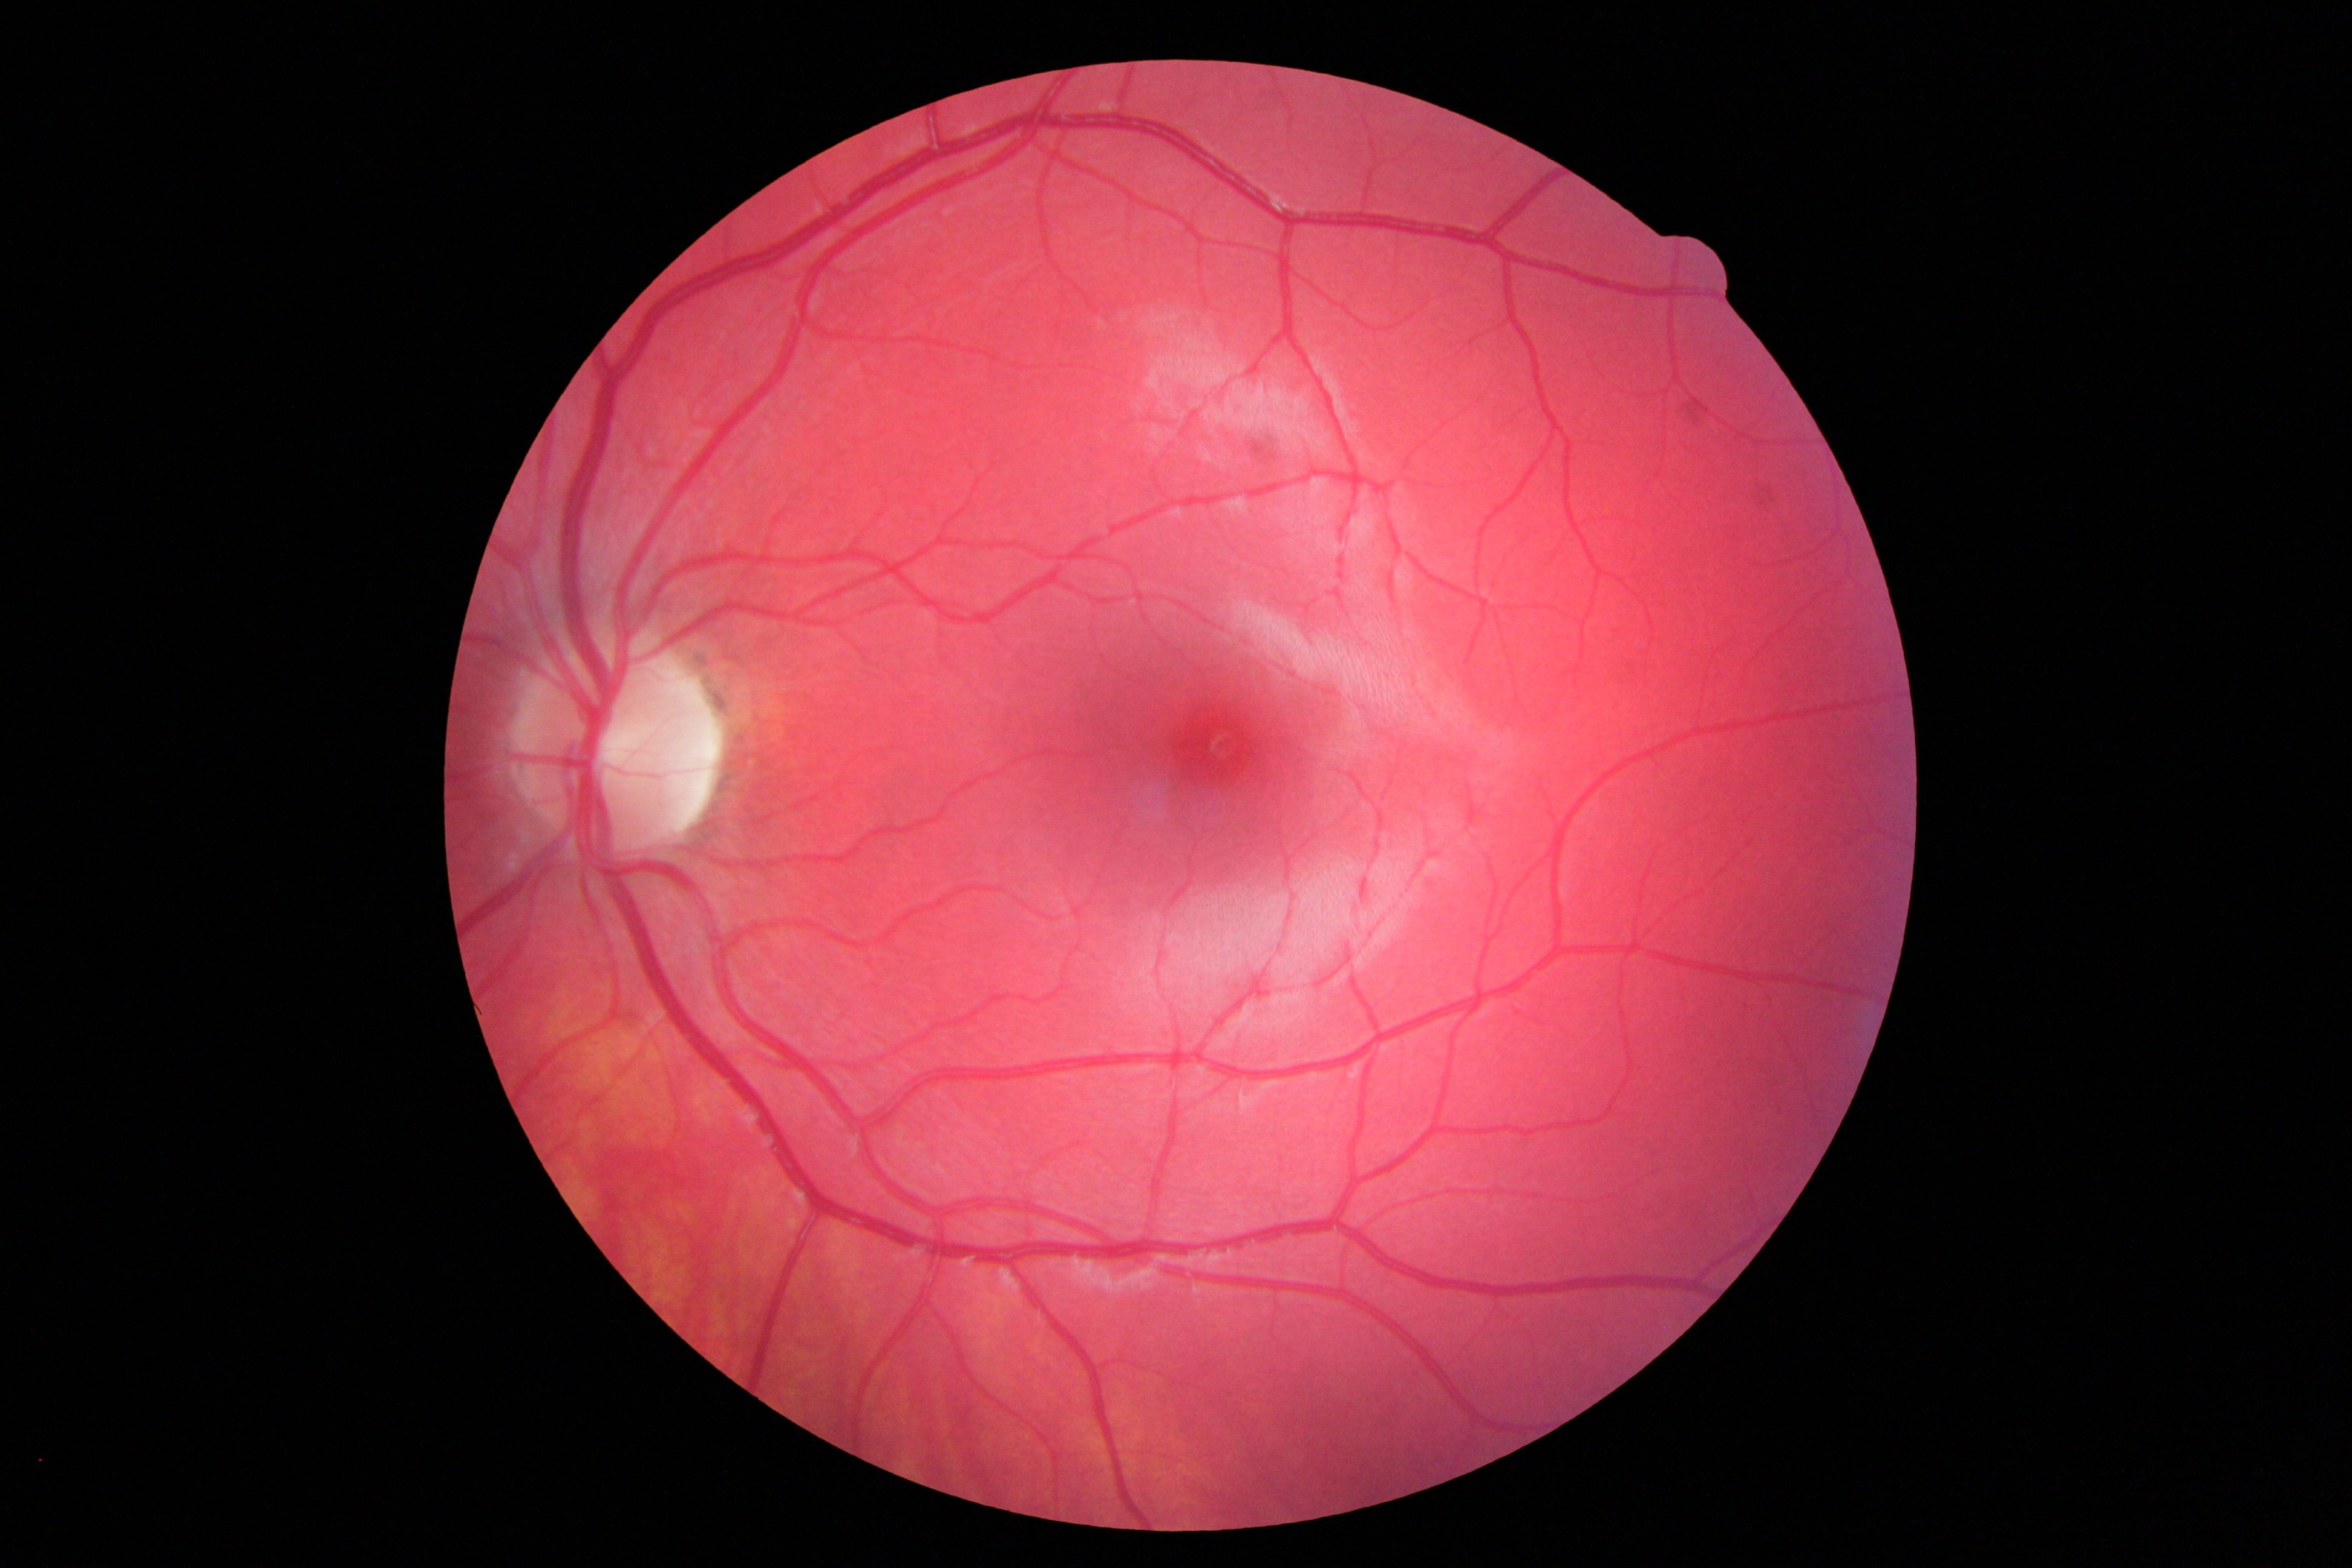
\includegraphics[width=\linewidth]{images/image.png}
  \caption{Originálny snímok}
  \label{fig:first-image}
\end{minipage}\hfill
\begin{minipage}{0.48\textwidth}
  \centering
  \includegraphics[width=\linewidth]{images/0011L1.png}
  \caption{Snímok po orezaní}
  \label{fig:second-image}
\end{minipage}
\caption{Porovnanie snímku pred a po pred-spracovaní}
\label{fig:two-images}
\end{figure}


\vspace{20px}

Trénovanie modelov bolo spustené na počítači s procesorom AMD Ryzen 7 7700x a grafickou kartou NVIDIA GeForce RTX 4070. Z trénovania, testovania a evaluácie boli vytvorené logy, ktoré sú uložené v priečinku \texttt{logs/}. V rámci presnosti jednotlivých modelov bola vytvorená nasledujúca tabuľka:
\begin{table}[h]
\centering
\begin{tabular}{|l|l|l|l|l|}
\hline
\textbf{Model} & \textbf{Presnosť} & \textbf{Trvanie trénovania} & \textbf{Dataset} & \textbf{Epochy} \\ \hline
ResNet18 & 0.82 & 206 minút & EyePACS & 30 \\ \hline
ResNet50 & 0.67 & 270 minút & EyePACS & 30 \\ \hline
DenseNet121 & 0.75 & 440 minút & EyePACS & 30 \\ \hline
ResNet18 & 0.63 & 12 minút & STRaDe & 30 \\ \hline
ResNet50 & 0.62 & 17 minút & STRaDe & 30 \\ \hline
DenseNet121 & 0.63 & 28 minút & STRaDe & 30 \\ \hline
\end{tabular}
\caption{Výsledky trénovania modelov na rôznych datasetoch}
\label{tab:train-results}
\end{table}

Ukážka výstupu trénovanie pre model \verb|densenet\_121| trénovaný 20 epochov je ukázaná prílohe \ref{lst:output}. Z tohto výstupu viem postupne vyčítať nasledovné: 
\begin{itemize}

    \item Parametre pri spustení
\begin{itemize}
    \item Zariadenie, ktoré bude na trénovanie použité (v tomto prípade grafická karta)
    \item Model, ktorý ide byť trénovaný (v tomto prípade model \verb|densenet121| 
    \item Vybraný \verb|criterion| a \verb|optimizer| 
\end{itemize}

\item Priebeh trénovania
\begin{itemize}
    \item Priebeh trénovania cez jeden epoch
    \item Priebeh validácie akuálne natrénovaného modelu
    \item Zobrazenie a porovnanie najlepšieho vs aktuálneho epochu
\end{itemize}

\item Priebeh testovania
\begin{itemize}
    \item Dĺžka \verb|test_loader-u| * 4 =  16252 snímkov na testovanie
    \item  Priebeh trénovania 
    \item Oznámenie o uložení výsledkov do súboru \verb|.csv|
\end{itemize}

\item Evaluácia
\begin{itemize}
    \item Zobrazenie súborov z ktorých sa ide pracovať a do ktorých sa ide ukladať
    \item Zobrazenie metrík, a to konkrétne:
\begin{itemize}
    \item \textbf{Accuracy}: Percentuálna miera správne klasifikovaných príkladov zo všetkých príkladov.
    \item \textbf{F1-Score}: Harmonický priemer presnosti (precision) a úplnosti (recall). Poskytuje vyváženú predstavu o výkone modelu.
    \item \textbf{AUC (Area Under the Curve)}: Plocha pod krivkou ROC (Receiver Operating Characteristic). Miera schopnosti modelu rozlišovať medzi triedami.
    \item \textbf{Sensitivity (Recall)}: Percentuálna miera správne identifikovaných príkladov pozitívnej triedy zo všetkých skutočných príkladov tejto triedy.
    \item \textbf{Precision}: Percentuálna miera správne identifikovaných príkladov pozitívnej triedy zo všetkých identifikovaných príkladov tejto triedy.
    \item \textbf{Specificity}: Percentuálna miera správne identifikovaných príkladov negatívnej triedy zo všetkých skutočných príkladov tejto triedy.
    \item \textbf{Micro-Precision}: Vypočítaná ako celková presnosť pre všetky triedy modelu.
    \item \textbf{Micro-Sensitivity}: Vypočítaná ako celková úplnosť pre všetky triedy modelu.
    \item \textbf{Micro-Specificity}: Vypočítaná ako celková špecificita pre všetky triedy modelu.
    \item \textbf{Micro-F1}: Vypočítaná ako celkový F1-skóre pre všetky triedy modelu.
    \item \textbf{TP (True Positives)}: Počet správne klasifikovaných pozitívnych príkladov.
    \item \textbf{TN (True Negatives)}: Počet správne klasifikovaných negatívnych príkladov.
    \item \textbf{FP (False Positives)}: Počet nesprávne klasifikovaných ako pozitívne príklady.
    \item \textbf{FN (False Negatives)}: Počet nesprávne klasifikovaných ako negatívne príklady.
\end{itemize}


\end{itemize}
\item Zobrazenie časových štatistík - doba trvania exekúcie daného módu/módov spustenia programu (bola použitá unixová utilita \verb|time|)
\end{itemize}

\section{Záver}
Cieľom práce bolo navrhnúť a vytvoriť nástroj, ktorého výsledkom je model neurónovej siete, ktorý analyzuje a následne klasifikuje obrázky sietnice do troch úrovní podľa kvality danej snímky. Táto funkcia môže urýchliť a spresniť kontrolu snímok sietnice pri pacientoch s chorobou, ktorú je možné identifikovať na týchto snímkach. Ako doplnok k práci je aj grafický program na manuálnu klasifikáciu kvality snímkov do generovanej tabuľky v súbore CSV.

Pred samotným trénovaním neurónovej siete bolo potrebné pred-pripraviť obrázky pre korektnú prácu s nimi. Po pripravení obrázkov je možné začať trénovanie modelu v jednotlivých epochách. Po validácii klasifikácie modelu každej epochy sa vyberie model s najväčšou úspešnosťou pri testovaní.

Najviac časovo náročnou časťou práce bolo práve trénovanie modelov, ktoré trvalo hodiny napriek využitiu modernej grafickej karty na akcelerovanie času tréningu.
Najúspešnejším modelom neurónovej siete bol model, ktorého výpis z trénovania sa nachádza v prílohe \ref{lst:output_best}. Tento model má úspešnosť správnej klasifikácie približne 82 \%. Úspešnosť modelu by mohla byť zvýšená prípadným zväčšením počtu epochov pri trénovaní. Aj napriek tomu je momentálna úspešnosť dostatočne vysoká na výrazné zrýchlenie a spresnenie kontroly snímok sietnice oka.
\pagebreak
\bibliographystyle{czechiso}
\renewcommand{\refname}{Zdroje}
\bibliography{ims}



\newpage
\section{Prílohy}

\begin{lstlisting}[breaklines=true, caption={Výstup z trénovania a evaluácie modelu pre model densenet121 a 20 epochov}, label={lst:output}]
==========================================
device:
GPU - NVIDIA GeForce RTX 4070
==========================================
model:
dense121_mcs
==========================================
criterion:
BCELoss()
==========================================
optimizer:
SGD (
Parameter Group 0
    dampening: 0
    differentiable: False
    foreach: None
    lr: 0.01
    maximize: False
    momentum: 0
    nesterov: False
    weight_decay: 0
)
==========================================
Total params: 28.86M


Training mode selected
Length of train_loader:  3136
Length of val_loader:  3136
Processing train Epoch -> 1 / 20 |################################| 3136 / 3136 | Time: 0.0 mins | Loss: 0.3288
Processing validation |################################| 3136 / 3136 | Time: 0.00 mins
Current Loss: 0.4153175348967162| Best Loss: inf at epoch: 0
Processing train Epoch -> 2 / 20 |################################| 3136 / 3136 | Time: 0.0 mins | Loss: 0.2988
Processing validation |################################| 3136 / 3136 | Time: 0.00 mins
Current Loss: 0.35579348392119364| Best Loss: 0.4153175348967162 at epoch: 0
... (remaining output)
Saving model with best loss: 0.24337111543673945 at epoch: 17
Model saved to ./result/densenet121.tar


Testing mode selected
Length of test_loader:  4063
Processing inference |################################| 4063 / 4063 | Time: 0.0 min.
Saving results to: data/densenet121.csv


Evaluating mode selected
Reading test labels from: data/test_labels.csv
Reading results from: data/densenet121.csv

Values classificated by model: dense121_mcs saved in data/densenet121.csv have following metrics:

Accuracy: 0.6749
F1: 0.5758
AUC: 0.8462
Sensitivity: 0.5943
Precision: 0.6371
Specificity: 0.7973
micro-Precision: 0.6749
micro-Sensitivity: 0.6749
micro-Specificity: 0.8375
micro-F1: 0.6749
tp: 3655.6667
tn: 9072.0000
fp: 1760.6667
fn: 1760.6667

________________________________________________________
Executed in  239.94 mins    fish           external
   usr time  298.86 mins    0.00 micros  298.86 mins
   sys time   39.89 mins  430.00 micros   39.89 mins
\end{lstlisting}

\newpage

\begin{lstlisting}[breaklines=true, caption={Výstup z trénovania a evaluácie modelu s najlepšími výsledkami pre model resnet18 a 30 epochov}, label={lst:output_best}]
==========================================
device:
GPU - NVIDIA GeForce RTX 4070
==========================================
model:
resnet18_mcs
==========================================
criterion:
BCELoss()
==========================================
optimizer:
SGD (
Parameter Group 0
    dampening: 0
    differentiable: False
    foreach: None
    lr: 0.01
    maximize: False
    momentum: 0
    nesterov: False
    weight_decay: 0
)
==========================================
Total params: 33.54M


Training mode selected
Length of train_loader:  3136
Length of val_loader:  3136
Processing train Epoch -> 1 / 30 |################################| 3136 / 3136 | Time: 0.0 mins | Loss: 0.5841
Processing validation |################################| 3136 / 3136 | Time: 0.00 mins
Current Loss: 0.3967082689668299| Best Loss: inf at epoch: 0
Processing train Epoch -> 2 / 30 |################################| 3136 / 3136 | Time: 0.0 mins | Loss: 0.5701
Processing validation |################################| 3136 / 3136 | Time: 0.00 mins
Current Loss: 0.3577176400469806| Best Loss: 0.3967082689668299 at epoch: 0
... (remaining output)
Saving model with best loss: 0.17737707616262405 at epoch: 29
Model saved to ./result/resnet_18.tar


Testing mode selected
Length of test_loader:  4063
Processing inference |################################| 4063 / 4063 | Time: 0.0 min.
Saving results to: data/resnet18.csv


Evaluating mode selected
Reading test labels from: data/test_labels.csv
Reading results from: data/resnet18.csv

Values classificated by model: resnet18_mcs saved in data/resnet18.csv have following metrics:

Accuracy: 0.8178
F1: 0.7784
AUC: 0.9358
Sensitivity: 0.7733
Precision: 0.7991
Specificity: 0.8964
micro-Precision: 0.8178
micro-Sensitivity: 0.8178
micro-Specificity: 0.9089
micro-F1: 0.8178
tp: 4429.6667
tn: 9846.0000
fp: 986.6667
fn: 986.6667

________________________________________________________
Executed in   72.04 mins    fish           external
   usr time  206.33 mins    0.00 micros  206.33 mins
   sys time   19.43 mins  430.00 micros   19.43 mins
   
\end{lstlisting}


\begin{figure}
    \centering
    \includegraphics[width=1\linewidth]{images/png (5).png}
    \caption{Architektúra DenseNet121 - vizualizovaná pomocou \href{https://pytorch.org/tutorials/intermediate/tensorboard_tutorial.html}{TensorBoard}}
    \label{fig:enter-label}
\end{figure}

\begin{figure}
    \centering
    \includegraphics[width=1\linewidth]{images/png (4).png}
    \caption{Architektúra ResNet18 - vizualizovaná pomocou \href{https://pytorch.org/tutorials/intermediate/tensorboard_tutorial.html}{TensorBoard}}
    \label{fig:enter-label}
\end{figure}

\begin{figure}
    \centering
    \includegraphics[width=1\linewidth]{images/png (6).png}
    \caption{Architektúra ResNet50 - vizualizovaná pomocou \href{https://pytorch.org/tutorials/intermediate/tensorboard_tutorial.html}{TensorBoard}}
    \label{fig:enter-label}
\end{figure}
\end{document}